\documentclass{beamer} %
\usepackage[utf8]{inputenc}
\usepackage{amsmath,bm,bbm} 
\usepackage{outlines}
\usepackage{times}
\usepackage{tikz}
\usepackage{amsmath}
\usepackage{verbatim}
\usepackage{graphicx}
\usepackage{booktabs}
\usetheme{CambridgeUS}
\usefonttheme{professionalfonts}
\usetikzlibrary{arrows,shapes}

%Apresentação do artigo base:
%Qual é o problema?
%Por que este problema é relevante?
%O que há de novo sendo apresentado?
%Quais são as grandes conclusões?

%Apresentação da Proposta de Mestrado:
%Título, nome e orientador
%Área de conhecimento
%Proposta da pesquisa do mestrado

\title[Séries Temporais]{Análise de Séries Temporais com Teoria da Informação}
\author{Eduarda T.\ C.\ Chagas$^{1}$, Roger Almeida$^{2}$ Alejandro C.\ Frery$^{3}$}

\institute{$^{1}$UFAL - Mestrado de Modelagem Computacional do Conhecimento\\
$^{2}$UFAL - Bacharelado em Engenharia da Computação\\
$^{3}$UFAL - Laboratório de Computação Científica e Análise Numérica}

\date{Janeiro 21,2018}

\AtBeginSection[]
{
  \begin{frame}<beamer>
    \frametitle{Sumário}
    \tableofcontents[currentsection,currentsubsection]
  \end{frame}
}

\begin{document}

\maketitle


% For every picture that defines or uses external nodes, you'll have to
% apply the 'remember picture' style. To avoid some typing, we'll apply
% the style to all pictures.
\tikzstyle{every picture}+=[remember picture]

% By default all math in TikZ nodes are set in inline mode. Change this to
% displaystyle so that we don't get small fractions.
\everymath{\displaystyle}

% Uncomment these lines for an automatically generated outline.
\begin{frame}{Sumário}
  \tableofcontents
\end{frame}

\section{Séries Temporais e Teoria da Informação}

\begin{frame}{Séries Temporais}

Tratam-se de conjuntos de dados, obtidos por meio de um processo observacional
ao longo de um determinado período de tempo.

\vspace{0.8cm}

\textbf{Áreas de aplicação}

\begin{itemize}
    \item Bolsa de valores
    \item Medicina
    \item Meteorologia
    \item Cotação de commodities
\end{itemize}

\end{frame}

\begin{frame}{Etapas do processo de análise}

\begin{itemize}
    \item \textbf{Simbolização}
    \begin{itemize}
        \item Processo de simbolização de Bandt e Pompe
    \end{itemize}
    \vspace{0.5cm}
    \item \textbf{Extração de informações}
    \begin{itemize}
        \item Entropias
        \item Distâncias estocásticas
        \item Complexidade estatística
    \end{itemize}
\end{itemize}

\end{frame}

\begin{frame}{Representação do espaço de probabilidade}

A tranformação de uma série temporal em uma distribuição de probabilidade $P$ permite avaliar o conteúdo informacional acerca da dinâmica do sistema e dos processos subjacentes, descrevendo-os de forma mensurável e observável.

\end{frame}

\begin{frame}{Simbolização de Bandt \& Pompe}

Seja a série $\bm x = (x_1, x_2, \dots, x_N)$, cada grupo de $D$ valores (não necessariamente adjacentes) será transformado em um padrão ordinal, para depois formar o histograma das suas ocorrências na série.
 
\end{frame}

\begin{frame}{Entropia de permutação}

Corresponde à medida quantitativa  de incerteza  de uma estrutura descrita por uma distribuição de probabilidade.

\begin{outline}
\1 Entropia de Shannon
  \begin{equation}
  	H(\bm h) = -\sum_{i}^{N} h_i \log h_i
  \end{equation}
 \end{outline}

\end{frame}

\begin{frame}{Distância Estocástica}

Mensurando a similaridade entre duas séries temporais, tal medida é calculada através da análise de suas respectivas distribuições de probabilidades

\end{frame}

\begin{frame}{Distância Estocástica}

\begin{table}[hbt]
\caption{Distâncias Estocásticas}\label{Tab:Distancias}
\centering
\begin{tabular}{lc}\toprule
Euclidiana					& $ \sqrt{\sum_i(q_i-p_i)^{2}}$\\
Manhattan					& $ \sum_{i}|q_i-p_i|$\\
Chebyshev					& $ \max_i\{|q_i-p_i|\}$\\
Kullback-Leibler			& $ \sum_{i}q_i \log\frac{q_i}{p_i}$\\
Jensen-Shannon				& $ \sum_{i} \Big(p_i \log\frac{p_i}{q_i} + q_i \log\frac{q_i}{p_i}\Big)$\\
Wotters						& $ \cos^{-1}\sum_{i} \sqrt{p_i q_i}$ \\
Bhattacharya				& $ -\log\sum_{i}\sqrt{p_i q_i}$ \\
\bottomrule
\end{tabular}
\end{table}

\end{frame}

\begin{frame}{Complexidade Estatística}

Procura encontrar estruturas de interação de dependência entre os elementos de uma dada série.

\vspace{0.8cm}

\begin{itemize}
\item Complexidade de Jensen-Shannon 
  \begin{equation}
  	C_{\text{JS}}(\bm h) = H_{\text{S}}(\bm h) . Q_{\text{JS}}(\bm h, \bm p)
  \end{equation}
\end{itemize}

\end{frame}

\begin{frame}{Séries temporais e a Teoria da informação}
    \begin{figure}
      \centering
       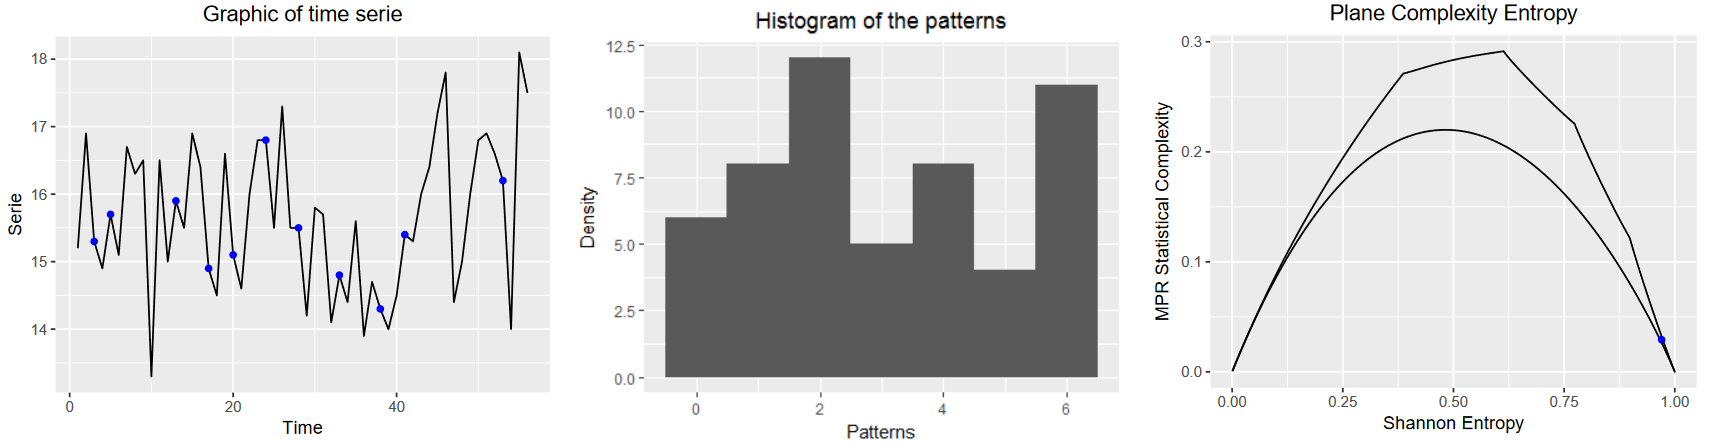
\includegraphics[width=10cm,height=3cm]{graphs.png}
    \end{figure}
\end{frame}

\section{Imputação de dados}

\begin{frame}{Problema Apresentado}
    \begin{figure}
      \centering
       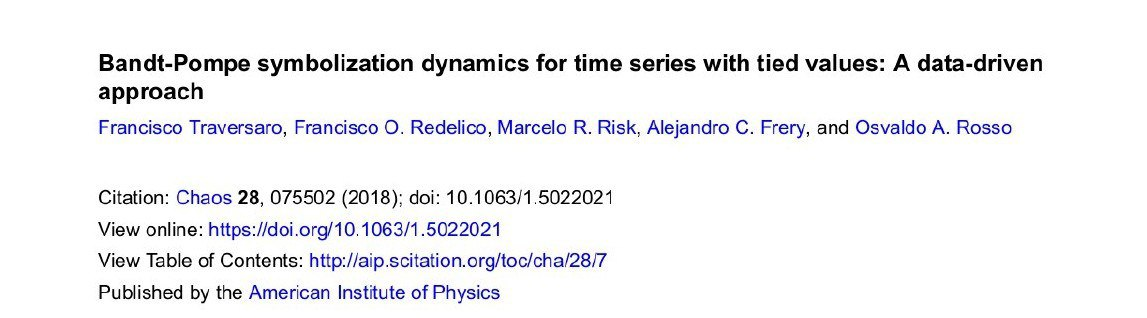
\includegraphics[width=10cm,height=3cm]{index.jpeg}
    \end{figure}
\end{frame}

\begin{frame}{Qual é o problema?}

Ao introduzir o conceito de entropia de permutação e o método de simbolização, Bandt e Pompe assumiram como condição inicial que os dados analisados consistiam de valores contínuos.

\vspace{0.8cm}

Análise de Séries Temporais discretas:

\begin{itemize}
    \item As séries são produzidas por geradores discretos de dados;
    \item Os dados serem discretizados como consequência da falta de precisão do dispositivo de medição de dados.
\end{itemize}

\end{frame}

\begin{frame}{O que há de novo sendo apresentado?}

\begin{itemize}
    \item Soluções computacionais para o problema de dados repetidos em séries temporais;
    \vspace{0.5cm}
    \item São apresentadas várias estratégias e mostrada as mais aptas a resolver este problema.
\end{itemize}

\end{frame}

\begin{frame}{Algoritmos de imputação de dados}

\textbf{Complete Case}

\begin{itemize}
    \item Método proposto originalmente por Bandt e Pompe, onde elimina do cálculo da probabilidade todos os padrões formados por elementos repetidos. 
\end{itemize}


\end{frame}

\begin{frame}{Algoritmos de imputação de dados}

\textbf{Time Ordered}

\begin{itemize}
    \item Se $x_{t1} = x_{t2}$ e $t_{1} < t_{2}$ então $x_{t1} < x_{t2}$.
\end{itemize}


\end{frame}

\begin{frame}{Algoritmos de imputação de dados}

\textbf{Random Imputation}

\begin{itemize}
    \item Sugere que padrões com valores iguais são o resultado de uma observação grosseira de padrões sem repetições originalmente, logo eles devem ser mapeados em símbolos correspondentes aos padrões originais com o mesmo peso probabilístico.
\end{itemize}


\end{frame}

\begin{frame}{Algoritmos de imputação de dados}

\textbf{Data Driven}

\begin{itemize}
    \item O método de imputação Data Driven (DDMI) consiste de uma metodologia semelhante ao Random Imputation mas, ao invés de adicionar uma perturbação aleatória com igual probabilidade para cada símbolo adequado, estas probabilidades são originadas de uma PDF previamente conhecida calculada por meio do método Complete Case.
\end{itemize}

\end{frame}

\begin{frame}{Conclusões}
    \begin{figure}
      \centering
       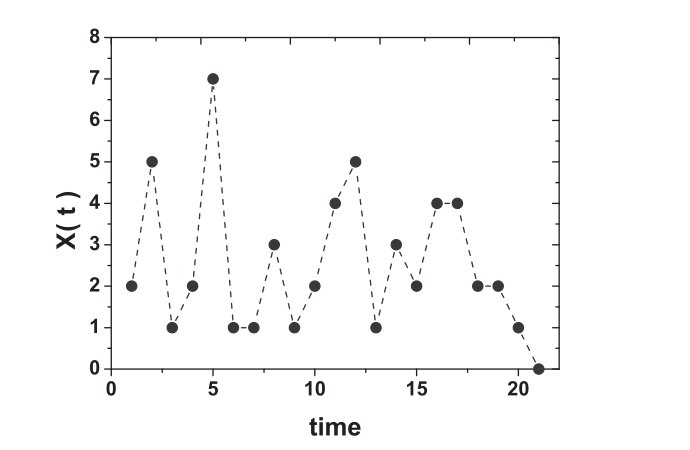
\includegraphics[width=8cm,height=5cm]{time.jpeg}
    \end{figure}
\end{frame}

\begin{frame}{Conclusões}
    \begin{figure}
      \centering
       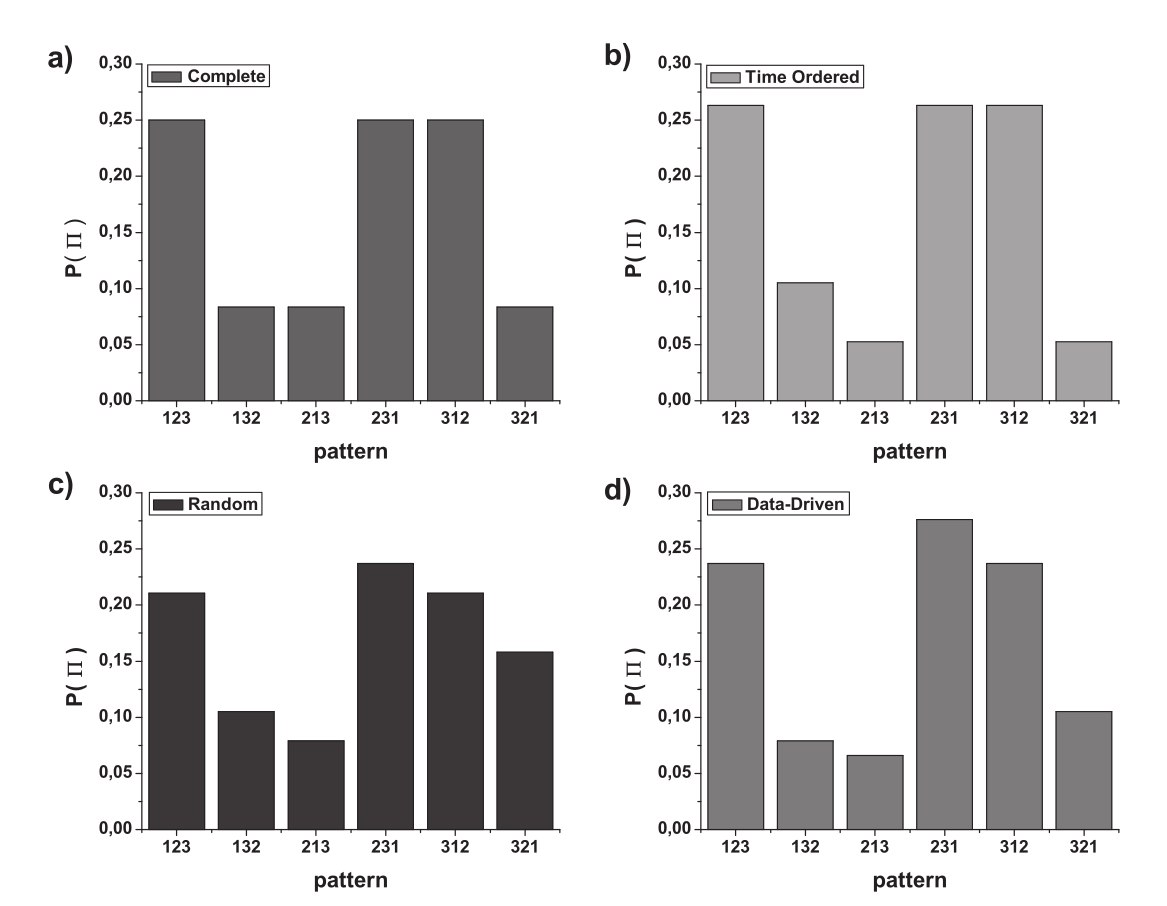
\includegraphics[width=10cm,height=6cm]{histogram.jpeg}
    \end{figure}
\end{frame}

\section{Proposta da pesquisa}

\begin{frame}{Pergunta de pesquisa}

Qual é o nível de pertubação $\psi$ tal que a técnica de imputação $\delta$ não consegue mais levar "próximo" do ponto $(h,c)$?

\end{frame}

\begin{frame}{Análise das técnicas no Plano HC}
    \begin{figure}
      \centering
       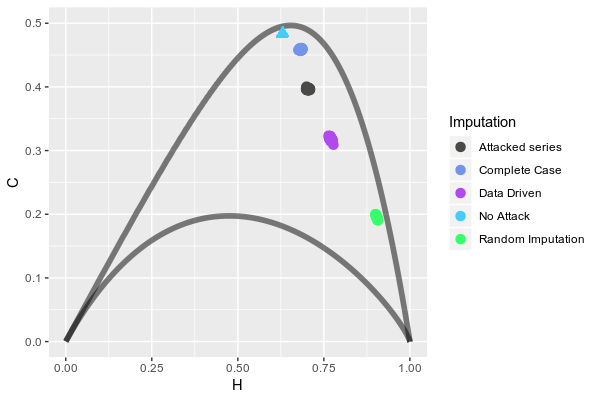
\includegraphics[width=9cm,height=6cm]{hcplane.png}
    \end{figure}
\end{frame}

\begin{frame}{Próximos passos}

Utilizar técnicas de SVM para comparar a eficiência das técnicas de imputação apresentadas.

\end{frame}

\end{document}